\documentclass[tikz,border=1pt]{standalone}
\usepackage{lmodern}\renewcommand{\familydefault}{\sfdefault}\usepackage[T1]{fontenc}
\usetikzlibrary{arrows.meta,positioning,calc}
\definecolor{ink}{HTML}{1A1A1A}\definecolor{gr}{HTML}{8A8A8A}\definecolor{grf}{HTML}{F2F2F2}
\definecolor{or}{HTML}{D55E00}\definecolor{orf}{HTML}{FDEEE6}\definecolor{gn}{HTML}{009E73}\definecolor{gnf}{HTML}{E6F5F0}
\definecolor{bl}{HTML}{0072B2}\definecolor{blf}{HTML}{E6F1F9}\definecolor{panel}{HTML}{FAFAFA}\definecolor{pline}{HTML}{C8C8C8}
\tikzset{
  box/.style={draw=gr,fill=grf,line width=0.6pt,rounded corners=2pt,minimum width=2.3cm,minimum height=0.95cm,text width=2.15cm,align=center,inner sep=2pt,font=\footnotesize,text=ink},
  mukv/.style={box,draw=or,fill=orf,line width=0.8pt},
  outc/.style={box,draw=gn,fill=gnf,line width=0.8pt},
  cbox/.style={box,minimum width=4.6cm,text width=4.4cm,minimum height=0.98cm},
  cmukv/.style={cbox,draw=or,fill=orf,line width=0.8pt},
  cout/.style={cbox,draw=gn,fill=gnf,line width=0.8pt},
  data/.style={-{Stealth[length=4pt,width=3.5pt]},line width=0.6pt,ink},
  ctrl/.style={-{Stealth[length=4pt,width=3.5pt]},line width=0.6pt,or,dashed},
  ctrlg/.style={-{Stealth[length=4pt,width=3.5pt]},line width=0.6pt,gr,dashed},
  heat/.style={-{Stealth[length=4pt,width=3.5pt]},line width=0.7pt,gr,dotted},
  meas/.style={-{Stealth[length=4pt,width=3.5pt]},line width=0.6pt,gn,dash dot},
  kv/.style={-{Stealth[length=4pt,width=3.5pt]},line width=0.6pt,bl},
  lab/.style={font=\scriptsize,inner sep=1pt,text=ink},
  stepn/.style={circle,fill=or,text=white,font=\bfseries\tiny,inner sep=1pt,minimum size=9pt},
  head/.style={font=\bfseries\scriptsize,inner sep=1pt}
}
\newcommand{\bx}[2]{\textbf{#1}\\[-1pt]{\scriptsize #2}}
\begin{document}
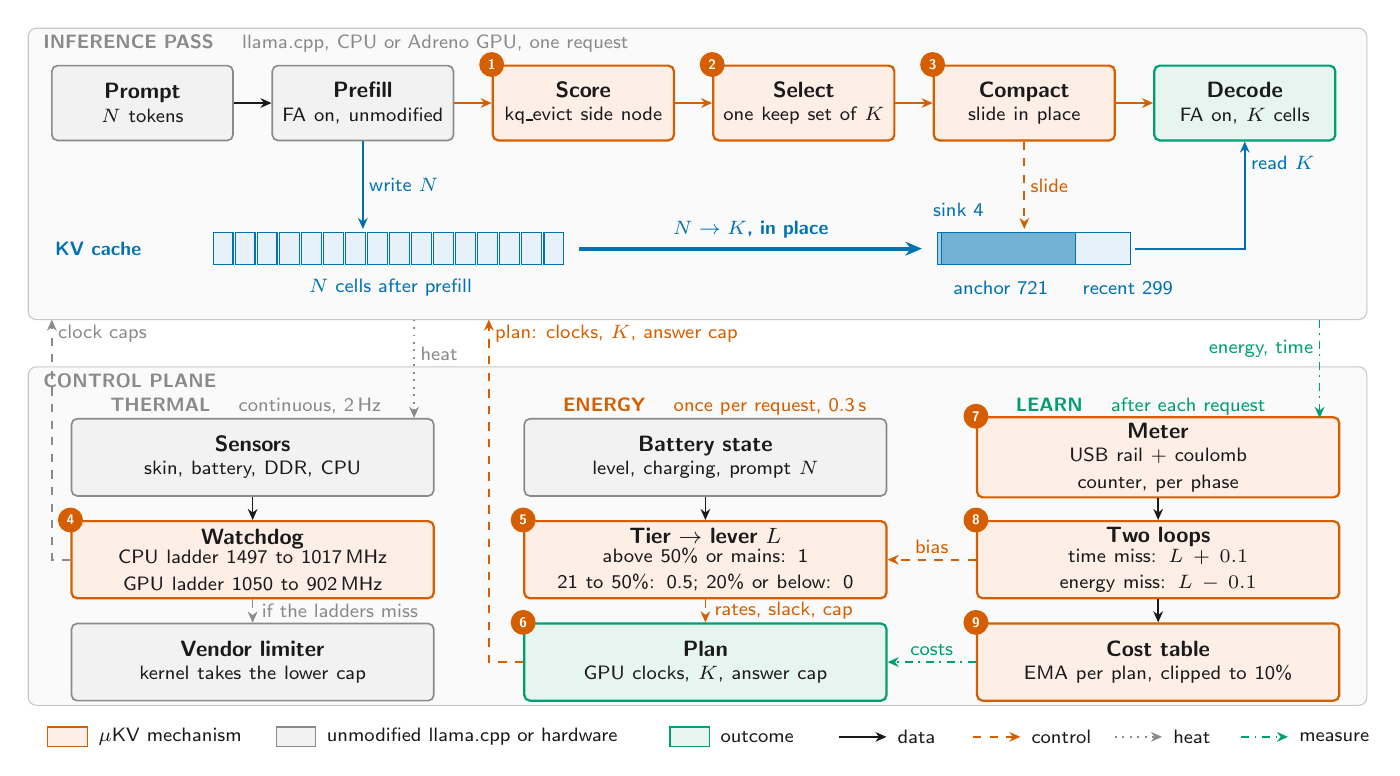
\begin{tikzpicture}[x=1cm,y=1cm]
% ---------------- panels ----------------
\fill[panel,draw=pline,rounded corners=3pt] (0,3.55) rectangle (17,7.25);
\fill[panel,draw=pline,rounded corners=3pt] (0,-1.35) rectangle (17,2.95);
\node[head,anchor=north west,text=gr] at (0.15,7.2) {INFERENCE PASS \quad {\mdseries llama.cpp, CPU or Adreno GPU, one request}};
\node[head,anchor=north west,text=gr] at (0.15,2.9) {CONTROL PLANE};
% ---------------- top row ----------------
\node[box] (prompt) at (1.45,6.3) {\bx{Prompt}{$N$ tokens}};
\node[box] (prefill) at (4.25,6.3) {\bx{Prefill}{FA on, unmodified}};
\node[mukv] (score) at (7.05,6.3) {\bx{Score}{kq\_evict side node}};
\node[mukv] (select) at (9.85,6.3) {\bx{Select}{one keep set of $K$}};
\node[mukv] (compact) at (12.65,6.3) {\bx{Compact}{slide in place}};
\node[outc] (decode) at (15.45,6.3) {\bx{Decode}{FA on, $K$ cells}};
\draw[data] (prompt) -- (prefill);
\draw[data,or] (prefill) -- (score);
\draw[data,or] (score) -- (select);
\draw[data,or] (select) -- (compact);
\draw[data,or] (compact) -- (decode);
\node[stepn] at (score.north west) {1};\node[stepn] at (select.north west) {2};\node[stepn] at (compact.north west) {3};
% ---------------- KV strip ----------------
\node[lab,text=bl,font=\bfseries\scriptsize,anchor=west] at (0.3,4.45) {KV cache};
\foreach \i in {0,...,15}{\fill[blf,draw=bl,line width=0.4pt] (2.35+\i*0.28,4.25) rectangle (2.35+\i*0.28+0.25,4.65);}
\node[lab,text=bl] at (4.6,3.95) {$N$ cells after prefill};
\draw[kv] (prefill.south) -- (4.25,4.7) node[lab,text=bl,midway,right=1pt] {write $N$};
\draw[kv,line width=1.4pt,-{Stealth[length=6pt,width=5pt]}] (7.0,4.45) -- (11.35,4.45) node[lab,text=bl,font=\bfseries\scriptsize,midway,above=2pt] {$N \to K$, in place};
% compacted strip proportional to the measured 4 / 721 / 299 split of K=1024
\fill[bl!35!white,draw=bl,line width=0.4pt] (11.55,4.25) rectangle (11.60,4.65);
\fill[bl!55!white,draw=bl,line width=0.4pt] (11.60,4.25) rectangle (13.30,4.65);
\fill[blf,draw=bl,line width=0.4pt] (13.30,4.25) rectangle (14.00,4.65);
\node[lab,text=bl,anchor=west] at (11.45,4.95) {sink 4};
\node[lab,text=bl] at (12.35,3.95) {anchor 721};
\node[lab,text=bl,anchor=west] at (13.35,3.95) {recent 299};
\draw[ctrl] (compact.south) -- (12.65,4.7) node[lab,text=or,midway,right=1pt] {slide};
\draw[kv] (14.05,4.45) -- (15.45,4.45) -- (decode.south) node[lab,text=bl,pos=0.8,right=1pt] {read $K$};
% ---------------- control plane columns ----------------
\node[head,text=gr,anchor=west] at (1.0,2.45) {THERMAL \quad {\mdseries continuous, 2\,Hz}};
\node[head,text=or,anchor=west] at (6.75,2.45) {ENERGY \quad {\mdseries once per request, 0.3\,s}};
\node[head,text=gn,anchor=west] at (12.5,2.45) {LEARN \quad {\mdseries after each request}};
\node[cbox] (sens) at (2.85,1.8) {\bx{Sensors}{skin, battery, DDR, CPU}};
\node[cmukv] (wd) at (2.85,0.5) {\bx{Watchdog}{CPU ladder 1497 to 1017\,MHz\\ GPU ladder 1050 to 902\,MHz}};
\node[cbox] (vend) at (2.85,-0.8) {\bx{Vendor limiter}{kernel takes the lower cap}};
\node[cbox] (batt) at (8.6,1.8) {\bx{Battery state}{level, charging, prompt $N$}};
\node[cmukv] (lever) at (8.6,0.5) {\bx{Tier $\to$ lever $L$}{above 50\% or mains: 1\\ 21 to 50\%: 0.5; 20\% or below: 0}};
\node[cout] (plan) at (8.6,-0.8) {\bx{Plan}{GPU clocks, $K$, answer cap}};
\node[cmukv] (meter) at (14.35,1.8) {\bx{Meter}{USB rail + coulomb counter, per phase}};
\node[cmukv] (loops) at (14.35,0.5) {\bx{Two loops}{time miss: $L+0.1$\\ energy miss: $L-0.1$}};
\node[cmukv] (table) at (14.35,-0.8) {\bx{Cost table}{EMA per plan, clipped to 10\%}};
\node[stepn] at (wd.north west) {4};\node[stepn] at (lever.north west) {5};\node[stepn] at (plan.north west) {6};
\node[stepn] at (meter.north west) {7};\node[stepn] at (loops.north west) {8};\node[stepn] at (table.north west) {9};
\draw[data] (sens) -- (wd);
\draw[ctrlg] (wd) -- (vend) node[lab,text=gr,midway,right=2pt] {if the ladders miss};
\draw[data] (batt) -- (lever);
\draw[ctrl] (lever) -- (plan) node[lab,text=or,midway,right=2pt] {rates, slack, cap};
\draw[data] (meter) -- (loops);
\draw[data] (loops) -- (table);
\draw[ctrl] (loops.west) -- (lever.east) node[lab,text=or,midway,above=1pt] {bias};
\draw[meas] (table.west) -- (plan.east) node[lab,text=gn,midway,above=1pt] {costs};
% vertical links between panels
\draw[heat] (4.9,3.55) -- (4.9,2.3) node[lab,text=gr,pos=0.35,right=1pt] {heat};
\draw[ctrlg] (wd.west) -- (0.3,0.5) -- (0.3,3.55) node[lab,text=gr,pos=0.94,right=1pt] {clock caps};
\draw[ctrl] (plan.west) -- (5.85,-0.8) -- (5.85,3.55) node[lab,text=or,pos=0.96,right=1pt] {plan: clocks, $K$, answer cap};
\draw[meas] (16.4,3.55) -- (16.4,2.3) node[lab,text=gn,pos=0.3,left=1pt] {energy, time};
% ---------------- legend ----------------
\node[draw=or,fill=orf,minimum width=0.5cm,minimum height=0.25cm,inner sep=0] (l1) at (0.5,-1.75) {};\node[lab,anchor=west] (l1t) at (0.85,-1.75) {$\mu$KV mechanism};
\node[draw=gr,fill=grf,minimum width=0.5cm,minimum height=0.25cm,inner sep=0] at (3.4,-1.75) {};\node[lab,anchor=west] at (3.75,-1.75) {unmodified llama.cpp or hardware};
\node[draw=gn,fill=gnf,minimum width=0.5cm,minimum height=0.25cm,inner sep=0] at (8.4,-1.75) {};\node[lab,anchor=west] at (8.75,-1.75) {outcome};
\draw[data] (10.3,-1.75) -- (10.9,-1.75);\node[lab,anchor=west] at (11.0,-1.75) {data};
\draw[ctrl] (12.0,-1.75) -- (12.6,-1.75);\node[lab,anchor=west] at (12.7,-1.75) {control};
\draw[heat] (13.8,-1.75) -- (14.4,-1.75);\node[lab,anchor=west] at (14.5,-1.75) {heat};
\draw[meas] (15.4,-1.75) -- (16.0,-1.75);\node[lab,anchor=west] at (16.1,-1.75) {measure};
\end{tikzpicture}
\end{document}
